\subsection{Nonlinear Optimization problem}
The objective is to minimize the following cost function:
\begin{align}
& \mbox{(C)}: \ \  V(x) = 1 + \left[ \begin{array}{cc} 1 & 2 \end{array} \right] x + \frac{1}{2} x^T \left[ \begin{array}{cc} 12 & 3 \\ 3 & 10 \end{array} \right] x  \\
& \hspace{2cm} + 10 \mbox{ln}(1+ x_1^4) \mbox{sin}(100x_1)+ 10 \mbox{ln}(1+x_2^4) \mbox{cos}(100x_2)  ; \ \  x \in \mathbb{R}^2  \nonumber
\end{align}
This is an unconstrained nonlinear optimization problem of the form:
\begin{align}
    V(x) = f(x)
\end{align}
where 
\begin{align}
    V \in \mathbb{R}
\end{align}
This can be solved using search algorithms: 
\begin{itemize}
    \item Steepest descent algorithms: 
    \item Secant algorithms: 
    \item Conjugate gradient method: 
\end{itemize}
\subsubsection{Solutions to unconstrained nonlinear problem using our python programs and matlab benchmark \textit{fminunc} function: }
All 4 algorithms converged to very close local minimal solutions for $x$ with a tolerance set to $tol =1e-4$ and the same initial value of column vector of $[0,0]^{T}$ as confirmed in the contour plot in figure 5. The gradient loss of the secant and algorithm converged to a minimum fastest of our Python-implemented subprograms while the conjugate gradient took longest to approach a minimum as can be seen in Figure 4. The Matlab program used the \textit{quasi newton} algorithm and quickly found a solution in 5 iterations.
The contour plot of the function $V(x)$ and the minimum solutions of $x$ derived from the 4 algorithms showed that 
\begin{table}[htbp]
\centering
\begin{center}
\begin{tabular}{|c|c|c|c|c|}
\hline
 & \textbf{Steepest Descent} & \textbf{Secant} &\textbf{Conjugate Method} &\textbf{\textit{Matlab}}\\
\hline
Iterations & 7 & 7 &8& 4 \\
\hline
$x$ & 
\begin{bmatrix}
-0.0177 \\
-0.0958  \\
\end{bmatrix}
&\begin{bmatrix}
 -0.0177 \\
 -0.0954\\
\end{bmatrix} & \begin{bmatrix}
 -0.01772 \\
 -0.0957 \\
\end{bmatrix} &\begin{bmatrix}
   0.080 \\
   -0.6607 \\
\end{bmatrix} \\
\hline 
\end{tabular}
\label{table:results}
\caption{Algorithm Performance}
\end{center}
\end{table}

\begin{figure}[h!]
\centering
\begin{subfigure}[t]{0.4\textwidth}
\centering
    \includegraphics[width=\textwidth]{images/python/sd-pB.eps}
\caption{}
\label{fig:Class distribution}
\end{subfigure}
\hfill 
\begin{subfigure}[t]{0.4\textwidth}
\centering
    \includegraphics[width=\textwidth]{images/python/sec-pB.eps}
    \caption{}
    \label{fig:TSNE}
\end{subfigure}
\hfill
\begin{subfigure}[t]{0.4\textwidth}
\centering
    \includegraphics[width=\textwidth]{images/python/cg-pB.eps}
    \caption{}
    \label{fig:TSNE}
\end{subfigure}
\hfill
\begin{subfigure}[t]{0.4\textwidth}
\centering
    \includegraphics[width=\textwidth]{images/matlab/1c_loss.eps}  
    \caption{}
    \label{fig:TSNE}
\end{subfigure}
\caption{(a): Steepest descent, (b): Secant method, (c): Conjugate gradient, (d): Matlab: \textit{fminunc - quasi-newton method}}
\end{figure}
\begin{figure}
    \centering
    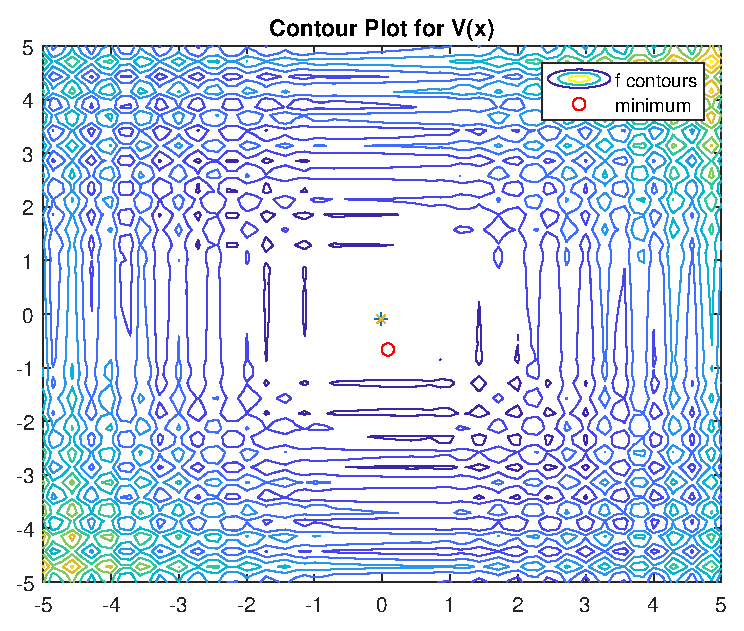
\includegraphics[width=0.4\textwidth]{images/matlab/matlab_1c.eps}
    \caption{Contour Plot for $V(x) = 1 + \left[ \begin{array}{cc} 1 & 2 \end{array} \right] x + \frac{1}{2} x^T \left[ \begin{array}{cc} 12 & 3 \\ 3 & 10 \end{array} \right] x  \hspace{2mm} + 10 \mbox{ln}(1+ x_1^4) \hspace{2mm}\mbox{sin}(100x_1)+ 10 \mbox{ln}(1+x_2^4) \mbox{cos}(100x_2)$}
\end{figure}